\documentclass{article}
\usepackage{amsmath}
\usepackage{graphicx}
\usepackage{geometry}
\usepackage{amsfonts}
\usepackage{amssymb}
\usepackage{graphicx}
\usepackage[utf8]{inputenc} %Spanish input                                      
\usepackage[T1]{fontenc} % Use 8-bit encoding that has 256 glyphs 
\usepackage[spanish, es-tabla]{babel}        
\usepackage{float}
\usepackage{lscape}
\usepackage{enumerate}
\usepackage{color}
\usepackage{algpseudocode}
\usepackage{mathtools}
\usepackage{wrapfig}
\usepackage{subfig}
\usepackage{cite} % para contraer referencias


%------------------------------------------------------------------------
\newtheorem{theorem}{Theorem}
\newtheorem{acknowledgement}[theorem]{Acknowledgement}
\newtheorem{algorithm}[theorem]{Algorithm}
\newtheorem{axiom}[theorem]{Axiom}
\newtheorem{case}[theorem]{Case}
\newtheorem{claim}[theorem]{Claim}
\newtheorem{conclusion}[theorem]{Conclusion}
\newtheorem{condition}[theorem]{Condition}
\newtheorem{conjecture}[theorem]{Conjecture}
\newtheorem{corollary}[theorem]{Corollary}
\newtheorem{criterion}[theorem]{Criterion}
\newtheorem{definition}[theorem]{Definition}
\newtheorem{example}[theorem]{Example}
\newtheorem{exercise}[theorem]{Exercise}
\newtheorem{lemma}[theorem]{Lemma}
\newtheorem{notation}[theorem]{Notation}
\newtheorem{problem}[theorem]{Problem}
\newtheorem{proposition}[theorem]{Proposition}
\newtheorem{remark}[theorem]{Remark}
\newtheorem{solution}[theorem]{Solution}
\newtheorem{summary}[theorem]{Summary}
\newenvironment{proof}[1][Proof]{\textbf{#1.} }{\ \rule{0.5em}{0.5em}}
\usepackage{fancyhdr}
\pagestyle{fancy}
\setlength{\textwidth}{7.0in}
\setlength{\oddsidemargin}{-0.35in}
\setlength{\topmargin}{-0.5in}
\setlength{\textheight}{9.0in}
\setlength{\parindent}{0.3in}
\setlength{\pdfpagewidth}{88.184mm}
\setlength{\pdfpageheight}{113.854mm}
\setlength{\footskip}{12.0pt}
\usepackage[hidelinks]{hyperref}
\usepackage{xstring}
\usepackage{listings}
\usepackage{lipsum}
\usepackage{courier}
\usepackage{multirow}
\usepackage{pdfpages}



\newcommand{\thelink}{\@empty}
\newcommand{\link}[2]{%
  \IfSubStr{#1}{:}{\renewcommand\thelink{#1}}{\renewcommand\thelink{#1:#2}}%
  \href{\thelink}{\texttt{#2}}%
}
%--------------------------------------------------------------
\geometry{
  a4paper,
  left=30mm,
  right=30mm,
  headheight=3cm,
  top=2.5cm,
  bottom=3.5cm,
  footskip=0cm
}
\begin{document}
\begin{titlepage}
\title{TSI PRACTICA 1}
\author{Pablo Huertas Arroyo}
\date{ \today }


\maketitle
\begin{figure}[h]
    \centering
    
\includegraphics[scale=4]{LogoUGR.png}
\end{figure}


\hspace{-1.7cm}
\newline Correo: \link{mailto}{phuertas@correo.ugr.es}
\newline DNI:77033078Y
\newline Grupo 3A, subgrupo 2
\newline Horario: Luneas de 17:30 a 19:30
\end{titlepage}

%\newpage
%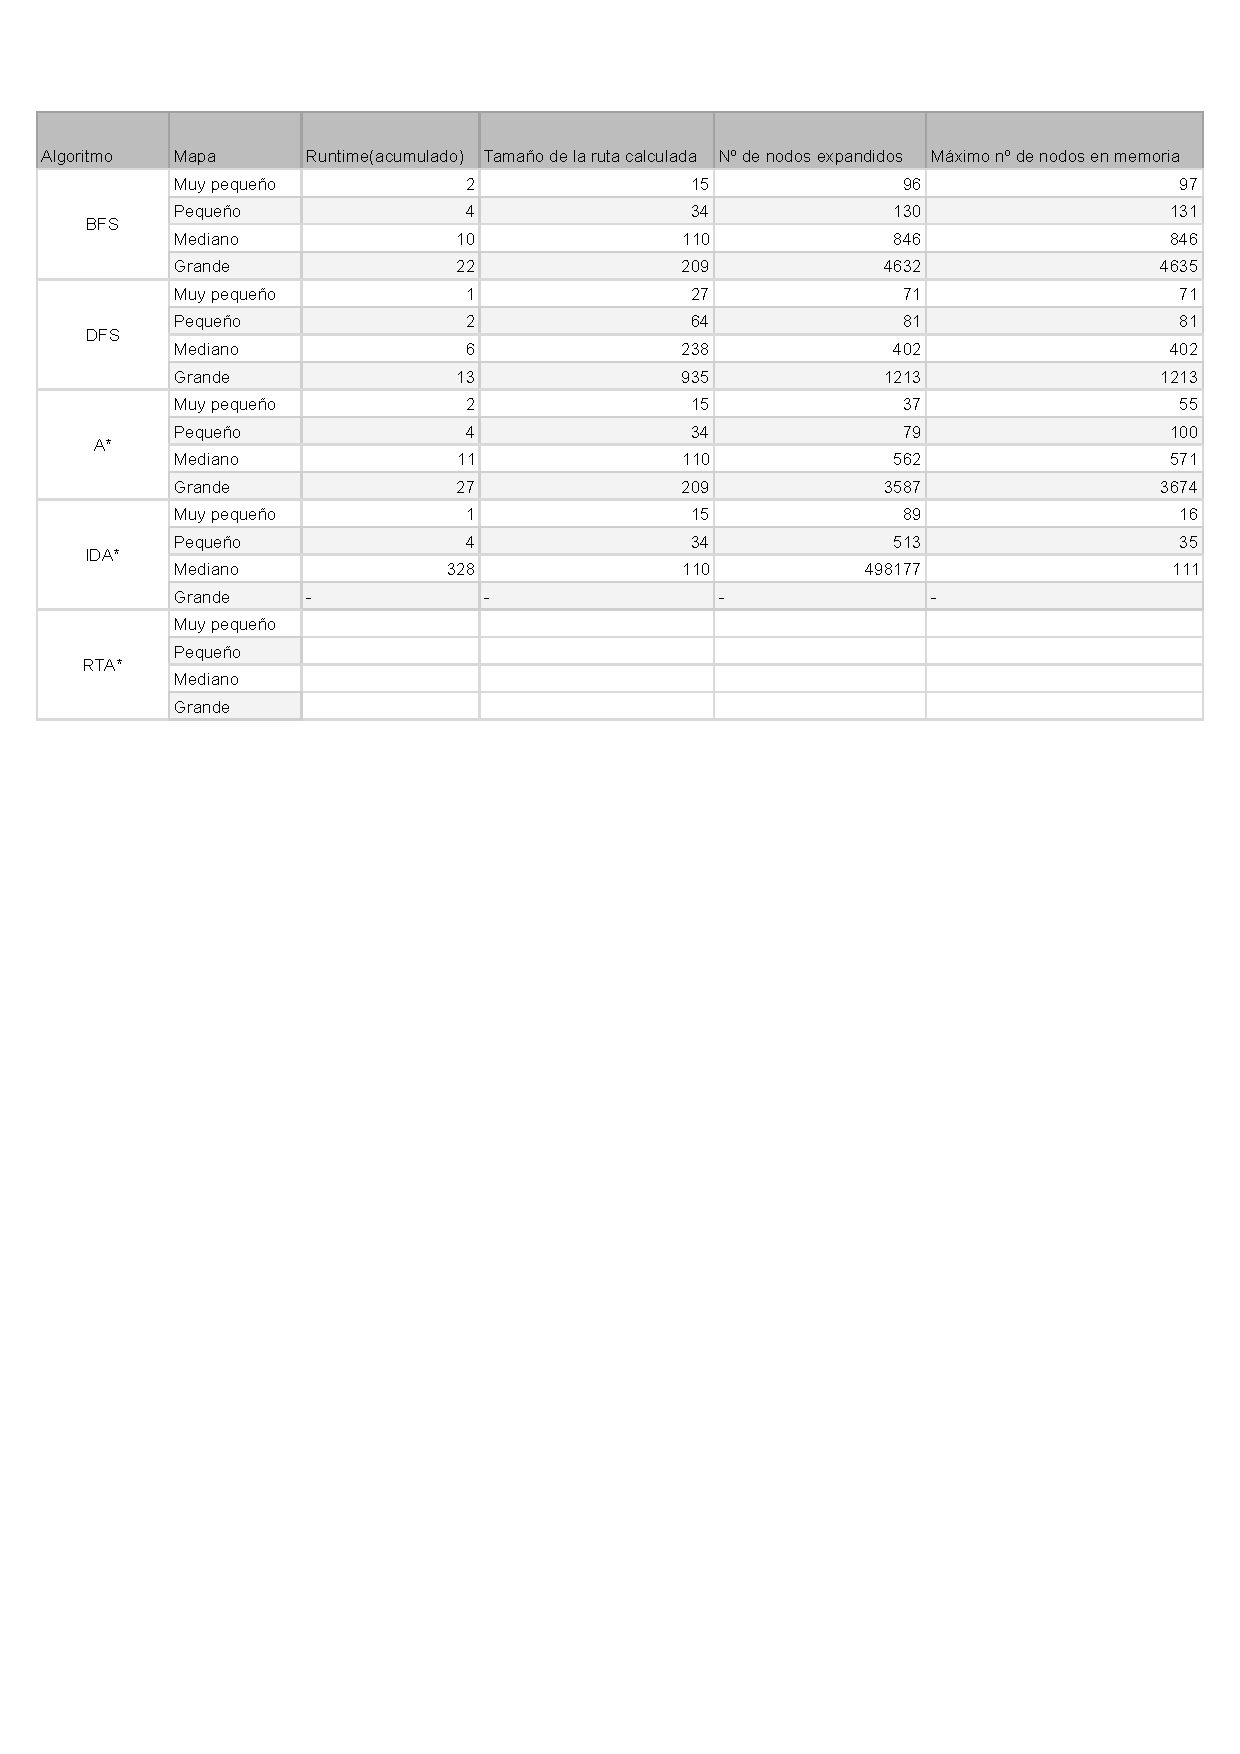
\includepdf[pages=-]{resultados.pdf}
%\vspace{10mm}




\section{\large{Cuestiones a resolver}}

\maketitle{\large{\textbf{Entre BFS y DFS, ¿qué algoritmo puede ser considerado más eficiente de cara a
encontrar el camino óptimo?}}}
\newline En este caso, el algoritmo más eficiente es el BFS, ya que es el que se encarga de encontrar el camino más corto 
al ir recorriendo todos los nodos nivel por nivel, terminando el algoritmo que encuentra el camino más corto.
En este problema nos encontramos con que todos los movimientos que se realizar tienen el mismo coste (1), por lo que 
en este caso el algoritmo BFS nos da el camino más corto y con menor coste.
En cambio, DFS nos da un camino de manera más rápida, pero no tiene por qué ser el camino más corto.

\vspace{5mm}
\maketitle{\large{\textbf{\newline ¿Se podría decir que A* es más eficiente que DFS?}}}
\newline Si nos referimos a tiempo, el algoritmo DFS tarda menos en encontrar un camino desde el nodo inicial hasta el nodo 
objetivo. Lo podemos observar en la tabla de resultados que en todos los mapas el tiempo empleado por el algoritmo DFS es menor 
que el tiempo empleado por el algoritmo A*.
El algoritmo A* calcula el camino óptimo, pero de una manera mucho más costosa que requiere de más tiempo.

\vspace{5mm}
\maketitle{\large{\textbf{\newline ¿Cuáles son las principales diferencias entre A* e IDA*? ¿En qué contextos es
más conveniente usar uno u otro?}}}
\newline A* es un algoritmo de búsqueda que, a través de una heurística, busca el camino más corto entre el nodo inicial y el nodo.
Almacena muchos más nodos en memoria que IDA*, ya que el algoritmo de búsqueda A* guarda en memoria dos listas, una de Abiertos y otra 
de Cerrados. \emph{Abiertos en mi caso una cola con prioridad, y Cerrados una tabla hash}.
IDA* usa el planteamiento heurístico de A*, pero este en vez de realizar un recorrido en anchura de los nodos generados, realiza un recorrido 
en profundidad. Con cada iteración no se incrementa la profundidad de los niveles, sino el costo total del camino.ç
IDA* no puede detectar estados repetidos ya que no cuenta con almacenamiento de estados como A*.
En contextos donde se necesite mayor rapidez, se recomienda usar A*, siempre y cuando la limitación de memoria no sea 
un problema. En estos casos, donde la memoria es escasa, se recomienda usar IDA*, ya que no requiere prácticamente de almacenamiento 
de estados.

\vspace{5mm}
\maketitle{\large{\textbf{\newline ¿Se podría decir que RTA* es más eficiente que A*?}}}
\newline No, RTA* es un algoritmo que en memoria solo almacena los estados que han sido visitados, y tiene un espacio local de búsqueda muy limitado.
Es decir, si nos imaginamos un pequeño robot que se mueve en una grilla de 10x10, y el sensor del robot tiene un alcance de 1 casilla, 
por cada paso que da el robot, solo podría ampliar su conocimiento de la grilla hasta un máximo de 4 casillas (suponiendo que puede ir hacia arriba, abajo, 
izquierda y derecha). El espacio local de aprendizaje sería la casilla del grid en la que se encuentra el robot, y que a medida que avanza puede ir 
aprendiendo más del entorno. Requiere de muy poca memoria, y en ocasiones puede ser bastante rápido, siempre y cuando no caiga en bucles intentando escapar de 
máximos locales.
A* sabemos que necesita mucha memoria, pero tiene la capacidad de calcular un camino completo, sin necesidad de replanificar, y además encontrará el camino óptimo,
siempre y cuando la heurística sea adecuada al problema.

\newpage \section{\large{Resultados}}
\begin{figure}[h]
  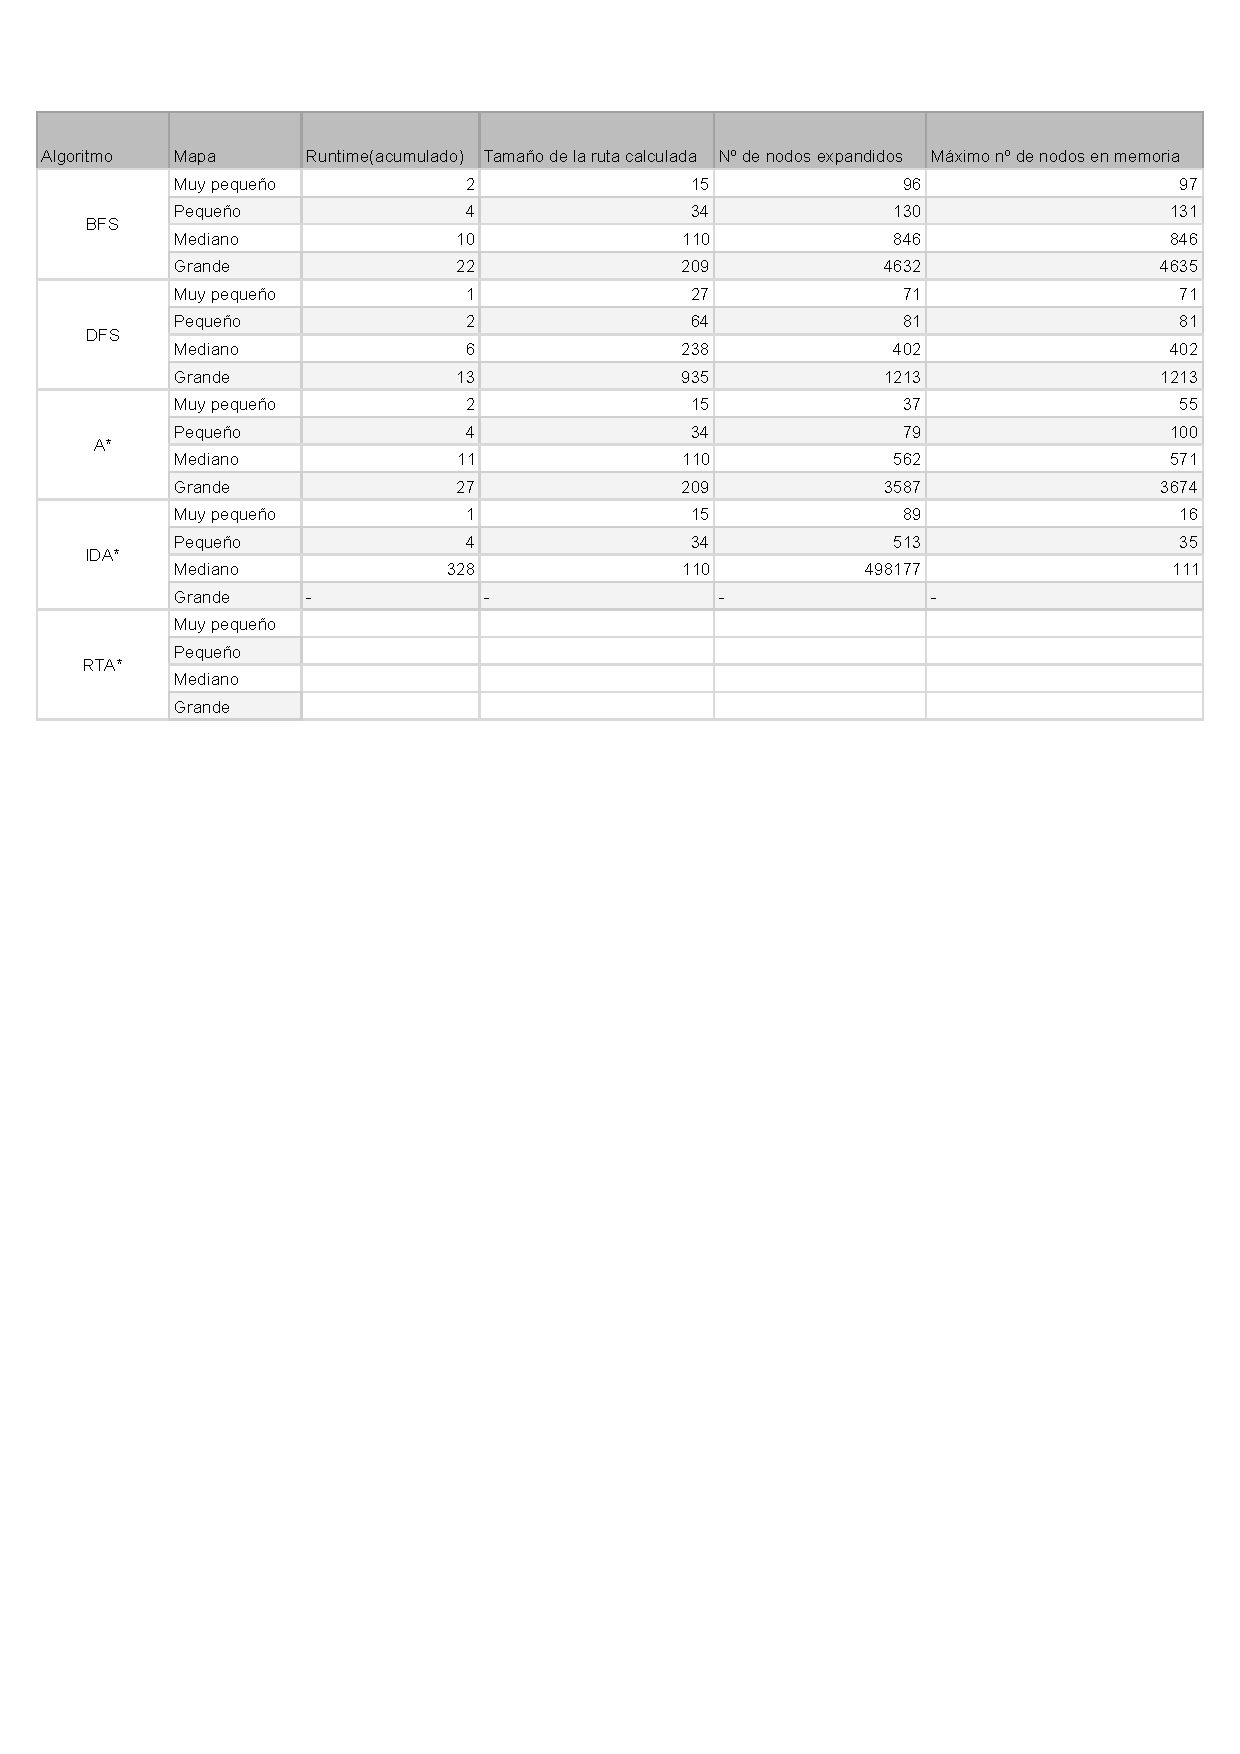
\includegraphics[scale=0.5]{resultados.pdf}
  \centering
  \caption{\textbf{Aclaración}: En el algoritmo IDA* en el mapa mediano se produce el Controller Disqualified, pero no 
  lo he puesto como Timeout(TO) porque creo que es diferente \newline El algoritmo RTA* no he podido implementarlo por tiempo, por lo que se 
  encuentra vacio}
\end{figure}
\end{document}